% See appendix 1 for a list of options for the xamk document class
\documentclass[minted, listings, pgfplots, bib]{xamk} % Use the xamk.cls document class
\addbibresource{main.bib} % Your bibliography BibTeX file goes here
\addbibresource{extra.bib}

% If "attach.zip" exists in the same directory, it will be attached to the output PDF.
% Anything meant to be written to the PDF should be within the document environment.
\begin{document}
	% Comments are written after a percent symbol. They are not compiled (i.e. rendered to the PDF).

	% Choose one of the following two title page formats. Remove percent symbols to start editing.

	% Format for title page of assignment/report/etc.
	%\xamkstudent{John Smith}{1234567}{ITMI17SP}
	%\xamkstudent{Jane Smith}{1234568}{ITMI17SP} % More than 1 student can be listed
	%\xamkstudent{Jake Smith}{1234569}{ITMI17SP} % The only limit is page space
	%\xamkpapertitle{Assignment 3}
	%\xamkpapersubtitle{Doing The Thing} % Optional
	%\xamkpapertype{Assignment}
	%\xamkcoursename{Computer Hardware}
    %\xamkpaperdate{2020}
	\maketitle % Creates title page with the preceding options (see xamk.cls)

	% Format for title page of thesis.
	%\xamkstudentname{John Smith}
	%\xamkpapertitle{This And That And The Other Thing}
	%\xamkpapersubtitle{Doing The Thing} % Optional
	%\xamkdegreetype{Master's Degree} % Optional, defaults to "Bachelor's Degree"
	%\xamkdegreeprogramme{Information Technology}
	%\xamkpaperdate{2020}
	%\maketitle[thesis] % Creates thesis title page with preceding options (see xamk.cls)

    % Format for the thesis abstract page (some info copied from thesis title page).
	%\xamkpagecount{99} % Number of pages (not including appendices)
	%\xamkappendixpagecount{9} % Number of appendix pages
	%\xamkthesiscommissioner{Random Company Ltd.}
	%\xamkthesissupervisor{Bob Smith}
	%\xamkthesiskeywords{documentation, model, thesis, report writing}
	%\xamkthesisabstractfile{thesis-abstract.tex} % Takes name of tex file containing abstract
    %\makethesisabstract % Creates thesis abstract page with preceding options (see xamk.cls)

	\tableofcontents % Automatically generates table of contents, based on sections/subsections/etc.

	% tex files can be imported with \input{} or \include{}
	% \input{} just imports the file, while \include{} also ensures page breaks before and after
	\section{Getting Started}

\subsection{"What am I supposed to do with these files?"}

The .tex files are what you edit.
What you want to get out of them is a PDF file.
This requires a \LaTeX\ compiler.
If you just want to get started and avoid The Complicated Stuff I'd recommend a free online compiler such as Overleaf (\url{https://www.overleaf.com/} \parencite{overleaf}).
Simply take the provided zip file and upload it with \textbf{New Project | Upload Project}.
Under the project menu, make sure to configure the TeX Live version to the latest.

\subsubsection{The Complicated Stuff}

For editing and compiling \LaTeX\ projects locally on your computer, I'd recommend VS Code with the \href{https://marketplace.visualstudio.com/items?itemName=James-Yu.latex-workshop}{LaTeX Workshop} extension \parencite{workshop}.
You'll also need a \TeX\ distribution (I'd recommend \href{https://www.tug.org/texlive/acquire-netinstall.html}{TeX Live} \parencite{texlive}).
If you don't do a full install, you'll need to manually install packages as compilation errors crop up.

For the minted package (used for code syntax highlighting), Python needs to be installed along with Python's \textbf{Pygments} package \parencite{pygmentize}.

Specify the following VS Code settings to enable the usage of the minted package, and to place generated files into an \texttt{out/} subfolder (try deleting this subfolder if you are experiencing weird compilation issues).
\begin{code}{json}[label=code:vscode-config]
"latex-workshop.latex.outDir": "%DIR%/out",
"latex-workshop.latex.tools": [{
    "name": "latexmk",
    "command": "latexmk",
    "args": ["--shell-escape", "-synctex=1", "-interaction=nonstopmode", "-pdf", "-outdir=%OUTDIR%", "%DOC%"]
}],
"latex-workshop.latex.recipes": [{
    "name": "latexmk",
    "tools": ["latexmk"]
}]
\end{code}

Restart VS Code, then with VS Code open the \texttt{xamk-template} folder.
Open the \texttt{xamk-template.tex} file.
A \TeX\ view should appear in the side bar.
Select \textbf{\TeX\ | Build LaTeX Project | Recipe: latexmk}, wait for the compilation to finish, then view the PDF with \textbf{\TeX\ | View LaTeX PDF}.

\subsection{Formatting}

{\centering\sc \large A Simple Sample \LaTeX\ File \parencite{formatting}\par}
\centerline{\sc Stupid Stuff I Wish Someone Had Told Me Four Years Ago}
\centerline{\it (Read the chapter1.tex file along with this or it won't make much sense)}

The first thing to realize about \LaTeX\ is that it is not ``WYSIWYG''.
In other words, it isn't a word processor; what you type into your .tex file is not what you'll see in your PDF.
For example, \LaTeX\ will      completely     ignore               extra    spaces    within                             a line of your .tex file.
Pressing return
in
the
middle
of
a
line
will not register in your PDF.
However, a double carriage-return is read as a paragraph break.

Like this.
But any carriage-returns after the first two will be completely ignored; in other words, you


can't

add






more




space


between




lines, no matter how many times you press return in your .tex file.

In order to add vertical space you have to use ``vspace''; for example, to get three lines of space you would type \verb|\vspace{3pc}| (``pc'' stands for ``pica'', a font-relative size), like this:
\vspace{3pc}

Notice that \LaTeX\ commands are always preceded by a backslash.
Some commands, like \verb|\vspace|, take arguments (here, a length) in curly brackets.

The second important thing to notice about \LaTeX\ is that you type in various ``environments''.
So far we've just been typing regular text (except for a few inescapable usages of \verb|\verb| and the centered, smallcaps, large title).
There are basically two ways that you can enter and/or exit an environment;
\vspace{0pc}

\centerline{this is the first way...}

\begin{center}
	this is the second way.
\end{center}

\noindent Actually there is one more way, used above; for example, {\sc this way}.
The way that you get in and out of environment varies depending on which kind of environment you want; for example, you use \verb|\underline| ``outside'', but \verb|\it| ``inside''; notice \underline{this} versus {\it this}.

The real power of \LaTeX\ (for us) is in the math environment.
You push and pop out of the math environment by typing \verb|$|.
For example, $2x^3 - 1 = 5$ is typed between dollar signs as \verb|$2x^3 - 1 = 5$|.
Perhaps a more interesting example is $\lim_{N \to \infty} \sum_{k=1}^N f(t_k) \Delta t$.

You can get a fancier, display-style math environment by enclosing your equation with double dollar signs.
This will center your equation, and display sub- and super-scripts in a more readable fashion:

$$\lim_{N \to \infty} \sum_{k=1}^N f(t_k) \Delta t$$

If you don't want your equation to be centered, but you want the nice indicies and all that, you can use \verb|\displaystyle| and get your formula ``in-line''; using our example this is $\displaystyle \lim_{N \to \infty} \sum_{k=1}^N f(t_k) \Delta t$.
However, this can screw up your line spacing a little bit.

There are many more things to know about \LaTeX\ and we can't possibly talk about them all here.
You can use \LaTeX\ to get tables, commutative diagrams, figures, aligned equations, cross-references, labels, matrices, and all manner of strange things into your documents.
You can control margins, spacing, alignment, {\it et cetera} to higher degrees of accuracy than the human eye can perceive.
You can waste entire days typesetting documents to be ``just so''.
\LaTeX\ can do anything, given you can find the package for the task.

The best way to learn \LaTeX\ is by example.
Get yourself a bunch of .tex files, see what kind of output they produce, and figure out how to modify them to do what you want.
The internet is full of instructions and examples for how to do various things in \LaTeX\ \parencite{tex-google}.
You'll need to do a lot of copy-pasting while learning how to use \LaTeX.
Good luck!

% Notice how each sentence starts from a new line, this helps with version control.
% Also notice the occasional ``<text>'', which creates the fancier quotation marks. % Imports chapter1.tex from the same directory as xamk-template.tex
	\section{Some Examples}

\subsection{Table}

Notice the missing | and \verb|\hline| in the chapter2.tex file and their effect.

% If you don't need a caption/label you can remove the table environment.
\begin{table}[H]
    %\centering
    % extra | before first l and missing | after the last l
    \begin{tabular}[b]{ || l | l  }
    	\hline % "\\" adds a linebreak, "\hline" adds a horizontal line
    	placeholder 1 & $(20.49 \pm 0.01)\si{mm}$ \\\hline
    	placeholder 2 & $(20.47 \pm 0.01)\si{mm}$ \\%\hline
    	placeholder 3 & $(18.63 \pm 0.01)\si{mm}$ \\\hline
    \end{tabular}
    \caption{An example table} % \citecaption can also be used in tables
    \label{tab:tabletest}
\end{table}

\subsection{Equation group}

For physics units, \verb|\si{}| can be used to easily distinguish units from variables (variables are italic).
% The "&"s control alignment. Try moving them around to adjust alignment.
\begin{align*}
    % _{} is used for subscript, ^{} is used for superscript
	V_{cuboid} &= w h l = 20.49\si{mm} \times 20.47\si{mm} \times 18.63\si{mm} \approx 7814\si{mm^{3}} \\ 
	% Notice how this \num{} converts its input into scientific notation
	G &= \num{6.673e-11}\si{N.m^{2}.kg^{-2}} \\ 
	% \num{} can also add those small spaces in large/small numbers
	\num{1000000} &= \num{1000000000000} \times \num{0.000001} \\
	x &= \frac{-b \pm \sqrt{b^2 - 4ac}}{2a} \\
	\int_{x^2 + y^2 \leq R^2} & f(x,y)\,dx\,dy
	    = \int_{\theta=0}^{2\pi} \int_{r=0}^R f(r\cos\theta,r\sin\theta) r\,dr\,d\theta.
	% If \\ was included after the last row it'd create an extra empty line of space below
\end{align*}
% Empty lines should be avoided around an align* environment, to preserve page space.
% Alternatively, a comment (even a "%" by itself) can be used.

\subsection{Graphics}

It's a cube with a hole through the top. Try changing the value of \texttt{cubex}.

% If you don't need the caption/label you can remove the figure environment.
\begin{figure}[H]
    %\centering
    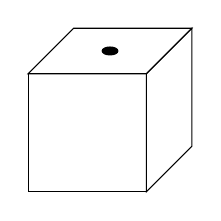
\begin{tikzpicture}
        \pgfmathsetmacro\cubex{1.5}
        \pgfmathsetmacro\cubey{1.5}
        \pgfmathsetmacro\cubez{1.5}
        \draw (0,0,0) -- ++(-\cubex,0,0) -- ++(0,-\cubey,0) -- ++(\cubex,0,0) -- cycle;
        \draw (0,0,0) -- ++(0,0,-\cubez) -- ++(0,-\cubey,0) -- ++(0,0,\cubez) -- cycle;
        \draw (0,0,0) -- ++(-\cubex,0,0) -- ++(0,0,-\cubez) -- ++(\cubex,0,0) -- cycle;
        \pgfmathsetmacro\circlex{\cubex/2}
        \pgfmathsetmacro\circlez{\cubez/2}
        \draw[fill=black] (-\circlex,0,-\circlez) ellipse (0.1 and 0.05);
    \end{tikzpicture}
    \citecaption{cube}{A cube drawn with TikZ} % 1st argument is the citation key, 2nd is the caption
    \label{fig:cube}
\end{figure}

\subsection{Graph}

% If you don't need the caption/label you can remove the figure environment.
\begin{figure}[H]
    %\centering
    \begin{tikzpicture}
    % Google "pgfplots gallery" to see examples of graphs and how to make them.
    % If you need negative numbers, add the "axis lines=middle" option to axis.
    \begin{axis}[
    xmin=0, xmax=1.2, ymin=0, ymax=2, % sets x-axis and y-axis limits
    xlabel={foo $a_1$ (\si{m.s^{-2}})}, % set x axis label
    ylabel={bar \\ $a_2$ (\si{m.s^{-2}})}] % set y axis label
    	\addplot+[only marks,error bars/.cd,
    	y dir=both,y explicit,
    	x dir=both,x explicit]
    	coordinates { % points
    		(0.1702, 0.376) +- (0.05, 0.25)
    		(0.2867, 0.552) +- (0.05, 0.25)
    		(0.3886, 0.724) +- (0.05, 0.25)
    		(0.4410, 0.891) +- (0.05, 0.25)
    		(0.5589, 1.05)  +- (0.05, 0.25)
    		(0.6659, 1.20)  +- (0.05, 0.25)
    		(0.7574, 1.35)  +- (0.05, 0.25)
    		(0.8580, 1.49)  +- (0.05, 0.25)
    		(0.9415, 1.63)  +- (0.05, 0.25)
    		(1.070,  1.77)  +- (0.05, 0.25)
    	};
    	% By default line domains are set to -5:5. You'll want to manually set them.
    	\addplot+[domain=0:2, color=black, mark=none, dotted] {2.2*x}; % dotted line
    	\addplot+[domain=0:2, color=black, mark=none, solid] {(1/0.541)*x}; % solid line
    	\addplot+[domain=0:2, color=black, mark=none, dashed] {1.5*x}; % dashed line
    \end{axis}
    \end{tikzpicture}
    \caption{A graph using TikZ's axis environment}
    \label{fig:fancygraph}
\end{figure}

\subsection{Monospace text}

Some Linux commands:
\begin{lstlisting}
wget http://tex.stackexchange.com
echo "is this thing working?" > test.txt
\end{lstlisting}

Some inlined paths: \lstinline{C:\Windows}, \lstinline{~/.bashrc} % \verb|| works as well

Some Python code with syntax highlighting:
% The starting line number is set with "firstnumber".
% {python} sets the language, use "pygmentize -L lexers" to get full list of supported languages.
\begin{minted}[firstnumber=11]{python}
def zip_gen(tuple_list):
    for index in range(min(len(tuple_list[0]), len(tuple_list[1]))):
        yield {tuple_list[0][index]: tuple_list[1][index]}
\end{minted}

\begin{comment} % This section is hidden due to the comment environment
Some C-sharp code with syntax highlighting:
% {csharp} sets syntax highlighting to C#.
\begin{minted}[firstnumber=11]{csharp}
private void StoreItemClicked(object sender, SelectionChangedEventArgs e) {
    if(Store.SelectedIndex != -1) {
        booksInCart.Add(booksInStore[Store.SelectedIndex]);
        booksInStore.RemoveAt(Store.SelectedIndex);
    }
    Refresh_ListBoxes();
}
\end{minted}
\end{comment}

\subsection{Image}

A figure containing an image and a caption:
% Figures (and tables) will reorder your layout if they're forced onto the next page.
% Using the [H] option for all figures and tables should prevent this problem from occurring.
% You could also manually reduce a figure's width or scale to fit within its page.
% If you don't need a caption/label for a figure you can use just the \includegraphics command.
\begin{figure}[H]
	%\centering % Uncomment to center the image and its caption
	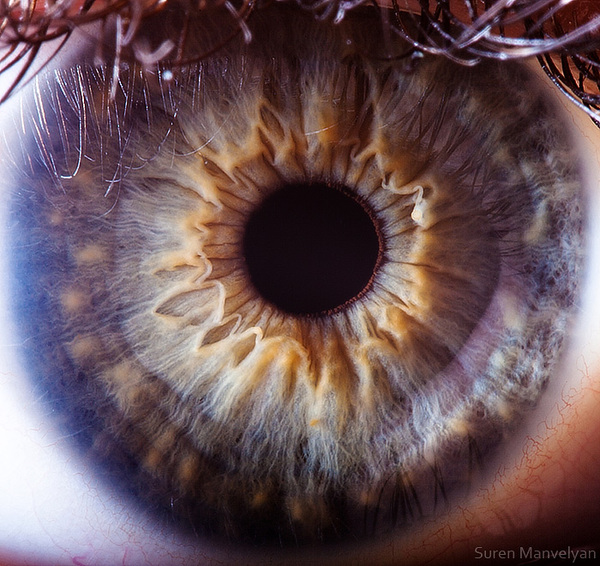
\includegraphics[width=0.8\linewidth]{eye.png}
	\citecaption{human-eye}{The human eye} % 1st argument is the citation key, 2nd is the caption
	\label{fig:human-eye}
\end{figure}


	% See appendix 1 for a description of this command's options
    \makebibliography[lof, lot] % Automatically generates the bibliography using biblatex

	% Appendix sections are expected to be within the appendices environment
	\begin{appendices}
        \section{Test Appendix 1}

\subsection{Standard Title Page}

\verb|\xamkstudentname{<student name>}{<student number>}{<group ID>}|\\
Specify your full name, student number, and group ID.
Can be used multiple times if the document should be attributed to multiple students.

\verb|\xamkpapertitle{<paper title>}|\\
Specify the title of the paper.

\verb|\xamkpapersubtitle{<paper subtitle>}|\\
Specify the subtitle of the paper (this command is optional).

\verb|\xamkpapertype{<paper type>}|\\
Specify the type of the paper (assignment, report, ect.)

\verb|\xamkcoursename{<course name>}|\\
Specify the name of the course the paper is written for.

\verb|\xamkpaperdate{<date>}|\\
Specify the year/date the paper was written in.

\verb|\maketitle|\\
Prints title page with preceding information (must be called after preceding commands).

\subsection{Thesis Title Page}

The following commands should be used before \verb|\maketitle[thesis]| is used.
the title, subtitle, and date commands are the same.

\verb|\xamkstudentname{<student name>}|\\
Replaces \verb|\xamkstudentname|.
Specify your full name (only takes one name).

\verb|\xamkthesistype{<degree type>}|\\
Specify your degree type.
Optional, defaults to "Bachelor's Degree".

\verb|\xamkdegreeprogramme{Information Technology}|\\

\verb|\maketitle[thesis]|\\
Prints thesis title page with preceding information (must be called after preceding commands).

\begin{comment}

\clearpage
\subsection{subsection 1}

\section{Test appendix 2}

\section{Test appendix 3}
\clearpage
\subsection{subsection 1}
\clearpage
\subsection{subsection 2}
\clearpage

\end{comment}

    \end{appendices}
\end{document}
